% НАСТРОЙКА СТРАНИЦЫ
\documentclass{article}
% Подключение Библиотек
% кирилица
\usepackage{ucs}
\usepackage[utf8x]{inputenc}
\usepackage[russian]{babel}
% изображения
\usepackage{graphicx}
\usepackage{capt-of} 
\usepackage{adjustbox} 
\usepackage{wrapfig}
% языки

% импорт
\usepackage{import}
\usepackage{example}
\usepackage{makeidx}
\usepackage{catchfilebetweentags}
% поворот
\usepackage{pdflscape}
\usepackage{afterpage}
\usepackage{rotating}
% текст 
\usepackage{amsmath}
\usepackage{amsfonts}
\usepackage{amssymb}
\usepackage{verbatim}
\usepackage{lipsum}
\immediate\write18{texcount -tex -sum  \jobname.tex > \jobname.wordcount.tex}
% код
\usepackage{listings}
% url
\usepackage{hyperref}
\usepackage{blindtext}
\usepackage{caption}
\usepackage{subcaption}
\usepackage{url}
\usepackage[T2A]{fontenc}
\usepackage[utf8]{inputenc}
\usepackage[russian]{babel}
% цвета
\usepackage{pagecolor,lipsum}
\usepackage{xcolor}
\usepackage[table]{xcolor}
\usepackage[dvipsnames]{xcolor}
\usepackage{xcolor,colortbl}

% Настройки Стиля
% страницы
\usepackage[left=20mm, right=10mm, top=20mm, bottom=20mm, nohead]{geometry}
\renewcommand{\baselinestretch}{1.50}
% ссылок
\hypersetup{
    colorlinks=true,
    linkcolor=blue,
    filecolor=magenta,      
    urlcolor=cyan,
    pdftitle={Overleaf Example},
    pdfpagemode=FullScreen,
    }
    
\urlstyle{same}
%% цвета
\definecolor{codegreen}{rgb}{0,0.6,0}
\definecolor{codegray}{rgb}{0.5,0.5,0.5}
\definecolor{codepurple}{rgb}{0.58,0,0.82}
\definecolor{backcolour}{rgb}{0.95,0.95,0.92}
\definecolor{mygreen}{rgb}{0.135,0.42,0.32}
\definecolor{anti-flashwhite}{rgb}{0.95, 0.95, 0.96}
\definecolor{ashgrey}{rgb}{0.7, 0.75, 0.71}
\definecolor{Gray}{gray}{0.85}
\definecolor{LightCyan}{rgb}{0.88,1,1}
% стиль кода с именем "mystyle1"
\lstdefinestyle{mystyle1}{
  backgroundcolor=\color{backcolour}, 
  commentstyle=\color{codegreen},
  keywordstyle=\color{magenta},
  numberstyle=\tiny\color{codegray},
  stringstyle=\color{codepurple},
  basicstyle=\ttfamily\footnotesize,
  breakatwhitespace=false,         
  breaklines=true,                 
  captionpos=b,                    
  keepspaces=true,                 
  numbers=left,                    
  numbersep=5pt,                  
  showspaces=false,                
  showstringspaces=false,
  showtabs=false,                  
  tabsize=2
}
% стиль кода с именем "mystyle2"
\lstdefinestyle{mystyle2}{
  frame=tb,
  language=Java,
  aboveskip=3mm,
  belowskip=3mm,
  showstringspaces=false,
  columns=flexible,
  basicstyle={\small\ttfamily},
  numbers=none,
  numberstyle=\tiny\color{gray},
  keywordstyle=\color{blue},
  commentstyle=\color{dkgreen},
  stringstyle=\color{mauve},
  breaklines=true,
  breakatwhitespace=true,
  tabsize=3
}
% стиль таблицы
\newcommand{\mc}[2]{\multicolumn{#1}{c}{#2}}
\newcolumntype{a}{>{\columncolor{Gray}}c}
\newcolumntype{b}{>{\columncolor{white}}c}
% Аннотация, Ключевые Слова И Ссылки
\providecommand{\keywords}[1] {
  \small	
  \textbf{\textit{Keywords---}} #1
}
\title{Лабораторная работа 1.2}
\author{Гордеев Никита  \\
        \small $^{1}$Петрозаводский государственный университет
}
\date{28 февраля 2023 г.} 
%положение figure
\makeatletter
\setlength{\@fptop}{0pt}
\makeatother


% ЛАБОРАТОРНАЯ РАБОТА 1
\begin{document}
% Задание 1 (Титульный Лист)
\maketitle
\begin{abstract}
Создание документа LaTeX. Создать исходный файл документа LaTeX со своими именем, отчеством и фамилией латинскими буквами...
\end{abstract} \hspace{10pt}
\keywords{создание, документа, latex}
\begin{thebibliography}{00}
\bibitem{b2} Разработка и анализ технической документации. // Кафедра Информатики и Математического Обеспечения. URL: https://kappa.cs.petrsu.ru/~chistyak/documentation/ (дата обращения: 28.02.2023).
\end{thebibliography}
\newpage
\tableofcontents
\clearpage

% Задание 2 (Альбомная Ориентация)
\afterpage{%
    \clearpage
    \thispagestyle{empty}
    \begin{landscape}
        \section{Альбомная Ориентация}
        Suspendisse at dolor tincidunt quam eleifend interdum venenatis vel odio. Quisque ornare molestie augue ut commodo. Cras sed mauris est. Cras vestibulum aliquet porttitor. Etiam leo metus, gravida ac sapien luctus, congue tempus diam. Orci varius natoque penatibus et magnis dis parturient montes, nascetur ridiculus mus. Suspendisse dictum massa et massa pulvinar, ac aliquam turpis blandit. Curabitur leo eros, venenatis sit amet justo eget, fringilla sollicitudin libero. Etiam sed ligula tortor. Nunc eu metus eu ipsum posuere dictum. Nullam lacinia convallis est, vitae tristique libero consectetur sit amet. Phasellus id blandit mauris, faucibus rutrum mi. Pellentesque at semper ipsum. \\

        \centering % Center table
        \begin{tabular}{llll}
            Column 1 & Column 2 & Column 3 & Column 4 \\
            A & B & C & D \\
            1 & 2 & 3 & 4 \\
            A & A & A & A \\
            Abc & Bca & Cab & Dac \\
            Aff & Bff & Cff & Dff \\
            
        \end{tabular}
        \captionof{table}{Table caption}% Add 'table' caption
    \end{landscape}
}
\clearpage


% Задание 3 (Многоуровневые Списки)
\section{Многоуровневые списки}

\subsection{Нумерованный многоуровневый список}
\begin{enumerate} 
  \item первый элемент первого уровня содержит список 
    \begin{enumerate} 
        \item элемент списка второго уровня
        \item второй элемент списка второго уровня
    \end{enumerate} 
  \item  второй элемент первого уровня
\end{enumerate}

\subsection{Маркированный многоуровневый список}
\begin{itemize}
  \item Level 0 Item 0 (первый уровень)
  \item Level 0 Item 1 (первый уровень)
  \begin{itemize}
    \item Level 1 Item
    \begin{itemize}
      \item Level 2 Item
      \begin{itemize}
        \item Level 3 Item
      \end{itemize}
    \end{itemize}
  \end{itemize}
\end{itemize}
\clearpage

% Задание 4 (Несколько Таблиц)
\section{Несколько Таблиц}

\subsection{Безрамочная таблица}
\begin{tabular}{c c c}
    A & B & C \\
    D & E & F \\
    G & H & I \\
\end{tabular}

\subsection{Таблица без горизонтальных линий}
\begin{tabular}{||l|c|r|p{6cm}||}
    Left & Center & Right & Paragraph \\
    1 & 1 & 1 & Lorem ipsum dolor sit amet, consectetuer adipiscing elit. \\
    12 & 12 & 12 & Ut purus elit, vestibulum ut, placerat ac, adipiscing vitae, felis. \\
    123 & 123 & 123 & Curabitur dictum gravidamauris. \\
\end{tabular}

\subsection{Не закрытая таблица}
\begin{tabular}{||l|c|r|p{6cm}||}
    \cline{1-3}
    Left & Center & Right & Paragraph \\
    \hline \hline
    1 & 1 & 1 & Lorem ipsum dolor sit amet, consectetuer adipiscing elit. \\
    \hline
    12 & 12 & 12 & Ut purus elit, vestibulum ut, placerat ac, adipiscing vitae, felis. \\
    \hline
    123 & 123 & 123 & Curabitur dictum gravidamauris. \\ [.3cm]
    \cline{4-4}
\end{tabular}

\subsection{Обычная таблица}
\begin{tabular}{|c|p{6cm}|}
    \hline
    Num & Top Aligned Paragraph\\
    \hline
    1 & Lorem ipsum dolor sit amet, consectetuer adipiscing elit. \\
    \hline
    12 & Ut purus elit, vestibulum ut, placerat ac, adipiscing vitae, felis. \\
    \hline
    123 & Curabitur dictum gravidamauris. \\
    \hline
\end{tabular}

\subsection{Повернутая таблица}
\begin{sidewaystable}
\centering
\caption{Sideways Table}
\begin{tabular}{|l|l|l|l|l|l|l|l|l| }
\hline
A2 & B2 & C1 & D1 & E1 & F1 & G1 & H1 & QWERTYQWERTY \\
\hline
A2 & B2 & C1 & D1 & E1 & F1 & G1 & H1 & QWERTYQWERTY \\
\hline
A2 & B2 & C1 & D1 & E1 & F1 & G1 & H1 & QWERTYQWERTY \\
\hline
A2 & B2 & C1 & D1 & E1 & F1 & G1 & H1 & QWERTYQWERTY \\
\hline
A2 & B2 & C1 & D1 & E1 & F1 & G1 & H1 & QWERTYQWERTY \\
\hline
\end{tabular}
\end{sidewaystable}
\clearpage

\subsection{Цветная таблица}
\begin{tabular}{|c|c|}
    \hline
    \cellcolor{purple!30}A & \cellcolor{pink!60}B \\
    \hline
    \cellcolor{red!40}C & \cellcolor{orange!50}D \\
    \hline
\end{tabular}

\subsection{Маленькая таблица}
\setlength{\arrayrulewidth}{1.5pt}
\begin{tabular}{|c|c|c|}
    \hline
    A & B & C \\
    \hline
    D & E & F \\
    \hline
    G & H & I \\
    \hline
\end{tabular}

\subsection{Объединённые по горизонтали ячейки в таблице}
\begin{tabular}{|l|l|l|}
    \hline
    \multicolumn{2}{|c|}{Multi-Column} & Column 3 \\
    \hline
    Column 1 & Column 2 & Column 3 \\
    \hline
\end{tabular}

\subsection{Объединённые по горизонтали и вертикали ячейки в таблице}
\begin{tabular}{|l|l|l|}
    \hline
    \multicolumn{2}{|c|}{\multirow{2}{*}{Multi-Row and Col}} & C1 \\
    \cline{3-3}
    \multicolumn{2}{|c|}{} & C2 \\
    \hline
    A3 & B3 & C3 \\
    \hline
\end{tabular}
\clearpage

% Задание 5 (Работа с цветом)
\section[Работа с текстом]{\textcolor{white}{Работа с} \label{second}
    \colorbox{ashgrey}{
        \textcolor{red}{ц}
        \textcolor{orange}{в}
        \textcolor{yellow}{е}
        \textcolor{green}{т}
        \textcolor{blue}{о}
        \textcolor{purple}{м}
        }
}
% цвет страницы
\pagecolor{mygreen}\afterpage{\nopagecolor}

% цвет текста
\textcolor{white}{This document presents several examples showing how to use the \texttt{xcolor} package to change the colour of \LaTeX{} page elements.}

% цвет списка
\begin{itemize}
\color{green}
\item First item
\item Second item
\color{orange}
\item \textcolor{orange}{\colorbox{black}{Third item}}
\item \textcolor{pink}{Fourth item}
\end{itemize}

% разделитель
\noindent
{\color{red} \rule{\linewidth}{0.5mm}}

% цвет текста
The background colour of text can also be \textcolor{red}{easily} set. For instance, you can change use an \colorbox{orange}{orange background} and then continue typing.

% фон блока
This is a sample text in black.
\textcolor{blue}{This is a sample text in blue.}
\textcolor{red}{This is a sample text in red.}
\textcolor{yellow}{This is a sample text in yellow.}
\textcolor{white}{\colorbox{orange}{This is a white sample text in orange colorbox.}}\\

% фон таблицы
\begin{tabular}{l | a | b | a | b}
\hline
\rowcolor{LightCyan}
\mc{1}{}  & \mc{1}{x} & \mc{1}{y} & \mc{1}{w} & \mc{1}{z} \\
\hline
variable 1 & a & b & c & d \\
variable 2 & a & b & c & d \\ \hline
\end{tabular}
\clearpage

% Задание 6 (Плавающее Окружение Figure)
\begin{figure}[t!]
\section{Плавающее Окружение Figure}
\centering
  \begin{minipage}[b]{0.4\textwidth}
    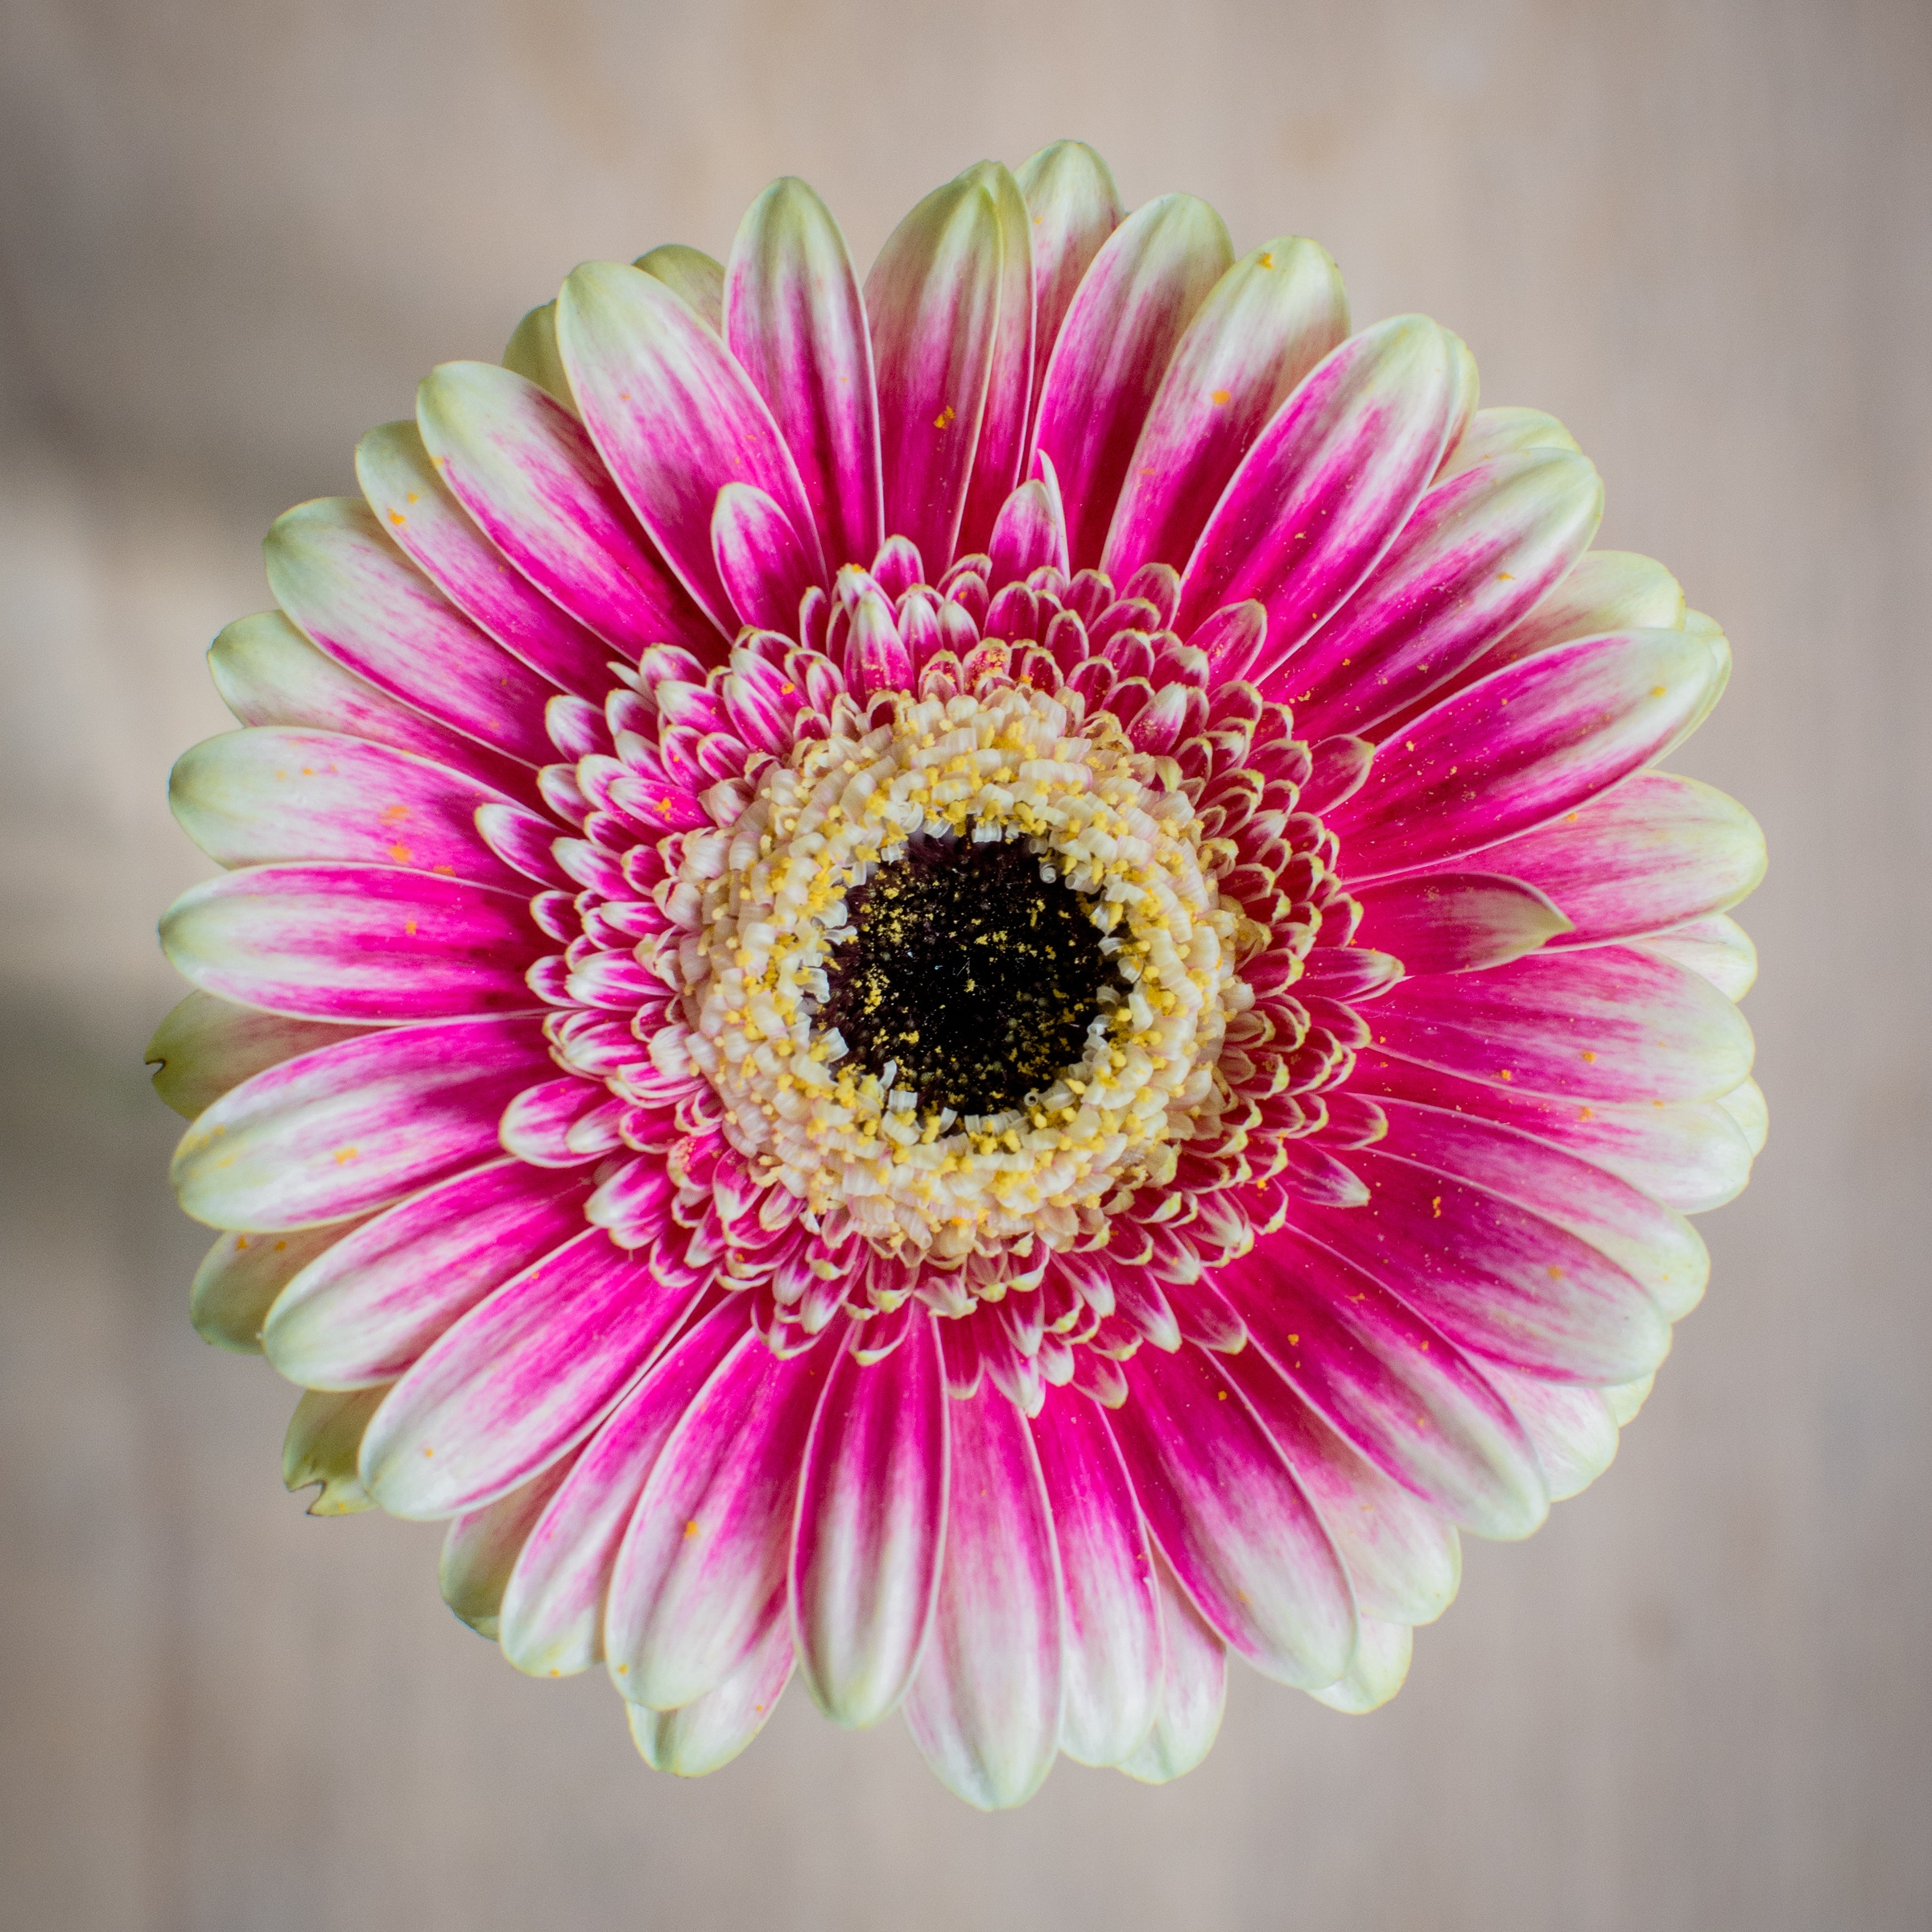
\includegraphics[width=\textwidth]{images/flower1.jpg}
    \caption{Flower one.}
  \end{minipage}
  \hfill
  \begin{minipage}[b]{0.4\textwidth}
    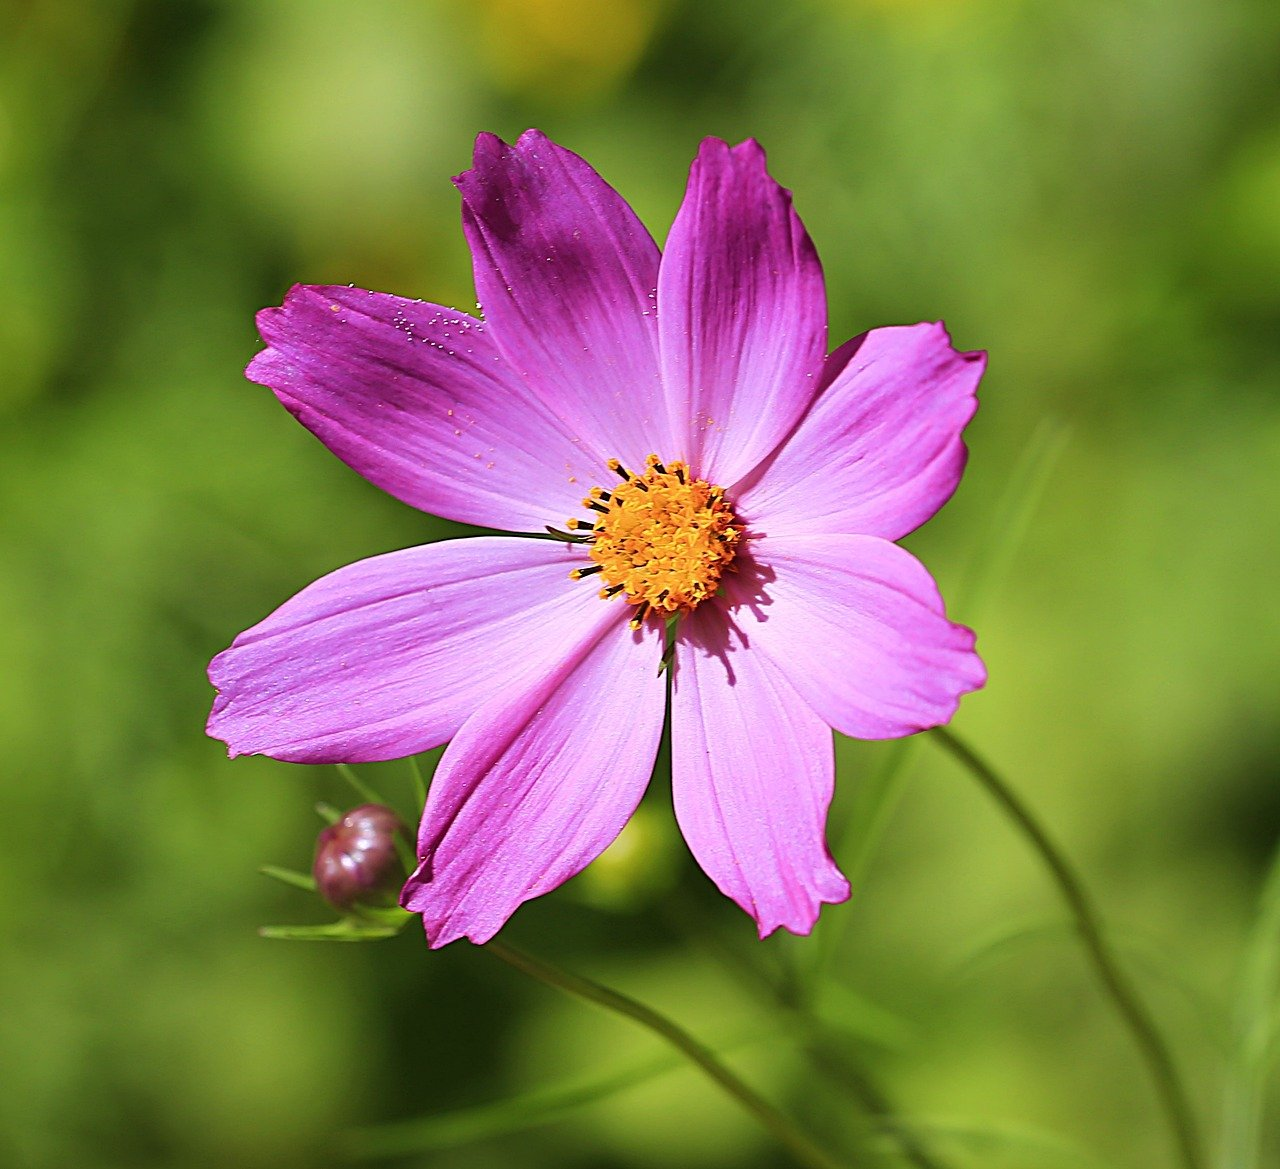
\includegraphics[width=\textwidth]{images/flower2.jpg}
    \caption{Flower two.}
  \end{minipage}
\end{figure}

% 
\begin{wrapfigure}{R}{0.3\textwidth}
\centering
\renewcommand{\figurename}{Fig.}

\includegraphics[width=0.25\textwidth]{images/frog.jpg}
\caption{\label{fig:frog1}This is a figure caption.}
\end{wrapfigure}

Lorem ipsum dolor sit amet, consectetuer adipiscing elit. Ut purus elit, vestibulum ut, placerat ac, adipiscing vitae, 
felis. Curabitur dictum gravida mauris. Nam arcu libero, nonummy eget, consectetuer id, vulputate a, magna. Donec vehicula augue eu neque. Pellentesque habitant morbi tristique senectus et netus et malesuada fames ac turpis egestas. Mauris ut leo. Cras viverra metus rhoncus sem. Nulla et lectus vestibulum urna fringilla ultrices.  Phasellus eu tellus sit amet tortor gravida placerat. Integer sapien est, iaculis in, pretium quis, viverra ac, nunc. Praesent eget sem vel leo ultrices bibendum. Aenean faucibus.
Morbi dolor nulla, malesuada eu, pulvinar at, mollis ac, nulla. Curabitur auctor semper nulla. Donec varius orci eget risus. Duis nibh mi, congue eu, accumsan eleifend, sagittis quis, diam. Duis eget orci sit amet orci dignissim rutrum.

\begin{wrapfigure}{L}{0.3\textwidth}
\centering

\includegraphics[width=0.25\textwidth]{images/frog.jpg}
\caption{\label{fig:frog2}This is a figure caption.}
\end{wrapfigure}

Nam dui ligula, fringilla a, euismod sodales, sollicitudin vel, wisi. Morbi auctor lorem non justo. Nam lacus libero, pretium at, lobortis vitae, ultricies et, tellus. Donec aliquet, tortor sed accumsan bibendum, erat ligula aliquet magna, vitae ornare odio metus a mi. Morbi ac orci et nisl hendrerit mollis. Suspendisse ut massa. Cras nec ante. Pellentesque a nulla. Cum sociis natoque penatibus et magnis dis parturient montes, nascetur ridiculus mus. Aliquam tincidunt urna. Nulla ullamcorper vestibulum turpis. Pellentesque cursus luctus mauris.

Nulla malesuada porttitor diam. Donec felis erat, congue non, volutpat at, tincidunt tristique, libero. Vivamus viverra fermentum felis. Donec nonummy pellentesque ante. Phasellus adipiscing semper elit. Proin fermentum massa ac quam. Sed diam turpis, molestie vitae, placerat a, molestie nec, leo. 
Maecenas lacinia. Nam ipsum ligula, eleifend at, accumsan nec, suscipit a, ipsum. Morbi blandit ligula feugiat magna. Nunc eleifend consequat lorem. Sed lacinia nulla vitae enim. Pellentesque tincidunt purus vel magna. Integer non enim. Praesent euismod nunc eu purus. Donec bibendum quam in tellus. Nullam cursus pulvinar lectus. Donec et mi. Nam vulputate metus eu enim. Vestibulum 
pellentesque felis eu massa.
\clearpage


% Задание 7 (Пакет Hyperref)
\section{Пакет Hyperref}

This will be an empty chapter and I will put some text here

\begin{equation}
\label{eq:1}
\sum_{i=0}^{\infty} a_i x^i
\end{equation}

The equation \ref{eq:1} shows a sum that is divergent. This formula will be later used on page \pageref{second}.

For further references see \href{https://kappa.cs.petrsu.ru/~chistyak/documentation/}{\textcolor{red}{cs.petrsu.ru}} or go to the next url: \url{https://tex.stackexchange.com/} or open the next file.

It's also possible to link directly any word or \hyperlink{thesentence}{any sentence} in your document.

If you read this text, you will get no information.  Really?  Is there no information?

For instance \hypertarget{thesentence}{this sentence}.



\clearpage



% Задание 8 (Фрагменты Программного Кода)
\section{Фрагменты Программного Кода}
\begin{lstlisting}[language=Python, caption=Python example]
import numpy as np
    
def incmatrix(genl1,genl2):
    m = len(genl1)
    n = len(genl2)
    M = None #to become the incidence matrix
    VT = np.zeros((n*m,1), int)  #dummy variable
    
    #compute the bitwise xor matrix
    M1 = bitxormatrix(genl1)
    M2 = np.triu(bitxormatrix(genl2),1) 

    for i in range(m-1):
        for j in range(i+1, m):
            [r,c] = np.where(M2 == M1[i,j])
            for k in range(len(r)):
                VT[(i)*n + r[k]] = 1;
                VT[(i)*n + c[k]] = 1;
                VT[(j)*n + r[k]] = 1;
                VT[(j)*n + c[k]] = 1;
                
                if M is None:
                    M = np.copy(VT)
                else:
                    M = np.concatenate((M, VT), 1)
                
                VT = np.zeros((n*m,1), int)
    
    return M
\end{lstlisting}

\clearpage
\lstset{style=mystyle1}
\begin{lstlisting}[language=Python, caption=Python example 2]
import numpy as np
    
def incmatrix(genl1,genl2):
    m = len(genl1)
    n = len(genl2)
    M = None #to become the incidence matrix
    VT = np.zeros((n*m,1), int)  #dummy variable
    
    #compute the bitwise xor matrix
    M1 = bitxormatrix(genl1)
    M2 = np.triu(bitxormatrix(genl2),1) 

    for i in range(m-1):
        for j in range(i+1, m):
            [r,c] = np.where(M2 == M1[i,j])
            for k in range(len(r)):
                VT[(i)*n + r[k]] = 1;
                VT[(i)*n + c[k]] = 1;
                VT[(j)*n + r[k]] = 1;
                VT[(j)*n + c[k]] = 1;
                
                if M is None:
                    M = np.copy(VT)
                else:
                    M = np.concatenate((M, VT), 1)
                
                VT = np.zeros((n*m,1), int)
    
    return M
\end{lstlisting}
\clearpage

\lstset{style=mystyle2}
\begin{lstlisting}[language=Python, caption=Python example 3]
import numpy as np
    
def incmatrix(genl1,genl2):
    m = len(genl1)
    n = len(genl2)
    M = None #to become the incidence matrix
    VT = np.zeros((n*m,1), int)  #dummy variable
    
    #compute the bitwise xor matrix
    M1 = bitxormatrix(genl1)
    M2 = np.triu(bitxormatrix(genl2),1) 

    for i in range(m-1):
        for j in range(i+1, m):
            [r,c] = np.where(M2 == M1[i,j])
            for k in range(len(r)):
                VT[(i)*n + r[k]] = 1;
                VT[(i)*n + c[k]] = 1;
                VT[(j)*n + r[k]] = 1;
                VT[(j)*n + c[k]] = 1;
                
                if M is None:
                    M = np.copy(VT)
                else:
                    M = np.concatenate((M, VT), 1)
                
                VT = np.zeros((n*m,1), int)
    
    return M
\end{lstlisting}
\clearpage

% Специальное Задание (Внешняя вставка)
\section*{Вставка внешних файлов}

\ExecuteMetaData[lorem.tex]{tag}

\vspace{10mm}
\begingroup
\obeylines
Lorem Ipsum - это текст-"рыба", часто используемый в печати и вэб-дизайне. Lorem Ipsum является стандартной "рыбой" для текстов на латинице с начала XVI века. 
В то время некий безымянный печатник создал большую коллекцию размеров и форм шрифтов, используя Lorem Ipsum для распечатки образцов. Lorem Ipsum не только успешно пережил без заметных изменений пять веков, но и перешагнул в электронный дизайн. Его популяризации в новое время послужили публикация листов Letraset с образцами Lorem Ipsum в 60-х годах и, в более недавнее время, программы электронной вёрстки типа Aldus PageMaker, в шаблонах которых используется Lorem Ipsum.
%
\endgroup%

\vspace{10mm}
\lstset{style=mystyle1}
\lstinputlisting[language=Python, firstline=17, lastline=24, firstnumber=17, numbers=left]{sort.py}

\clearpage

% Материалы
\begin{thebibliography}{100} 
\import{./}{bibliography.tex}
\end{thebibliography}

\end{document}
